\documentclass[twoside,UTF8]{EPURapport}
\usepackage{listings}

%\renewcommand{\lstlistlistingname}{Liste des codes}
%\renewcommand{\lstlistingname}{Code}

%\addextratables{%
%	\lstlistoflistings
%}

%\swapAuthorsAndSupervisors




\thedocument{Rapport de Projet}{Batching et optimisation des trajectoires de picking dans un centre d'entreposage}{Batching et picking}

\grade{Département Informatique\\ 3\ieme{} année\\ 2008 - 2009}

\authors{%
	\category{Étudiants}{%
		\name{Shimeng ZHANG} \mail{shimeng.zhang@etu.univ-tours.fr}
		\name{Natacha MARLIO-MARETTE} \mail{natacha.marlio-marette@etu.univ-tours.fr}
	}
	\details{DI3 2012 - 2013}
}

\supervisors{%
	\category{Encadrants}{%
		\name{Ameur SOUKHAL} \mail{ameur.soukhal@univ-tours.fr}
	}
	\details{Université François-Rabelais, Tours}
}

\abstracts{Ce projet de troisième année porte sur le batching et l'optimisation des trajectoires d'un chariot dans un centre d'entreposage. Deux heuristiques différentes ont été réalisée suivant la méthode \textit{Cluster First Root Second} et la méthode \textit{Root First Cluster Second}. Puis une série de tests ont été effectuée pour déterminer l'heuristique la plus performante.}
{Batching, Picking, Problème du voyageur de commerce, Problème de tournée de véhicules, NP-complet, Cluster First Root Second, Root First Cluster Second}
{This project is about batching and optimization of path from a wagon in a stocking center. Two differents heuristics exist to solve this problem : Cluster First Root Second and Root First Cluster Second. A set of tests were realised to determinate the most efficient heuristic. }
{Batching, Picking, Travelling Salesman Problem, Vehicle Routing Problem, NP-complete, Cluster First Root Seocnd, Root First Cluster Second}






\begin{document}

%%%%%%%%%%%%%%%%%%%% INTRODUCTION %%%%%%%%%%%%%%%%%%%%

\chapter{Introduction}

\paragraph{}
Le problème d'optimisation de la tournée de chariots dans un entrepôt de façon à récupérer des produits est un problème NP-complet, c'est à dire qu'il est possible de vérifier une solution en un temps polynomial. Ce problème peut soit être de type VRP (Vehicle Routing Problem) s'il y a plusieurs chariots de capacité différentes ou de type TSP (Travelling Salesman Problem) s'il n'y a qu'un chariot de capacité unique. 
\paragraph{}
Le problème du voyageur de commerce consiste à trouver le plus court chemin reliant un ensemble de points séparés par des distances connues en passant une fois seulement par chacun d'eux. Il n'existe pas de méthodes de résolution permettant d'obtenir des solutions exactes en un temps raisonnable pour de grandes instances car pour ces instances on se retrouve face à une explosion combinatoire.
\paragraph{}
Le problème de tournée de véhicules est une classe de problème de recherche opérationnelle et d'optimisation combinatoire. Il consiste à déterminer par exemple les tournées de plusieurs véhicules afin de livrer une liste de clients ou de réaliser des tournées d'interventions (réparation, contrôle, maintenance) ou de visites (commerciales, médicales, etc...). On peut rajouter quelques contraintes, telles que la capacité des véhicules qui peut être limitée, ou aux ressources et aux clients en fonctions des disponibilités, localisations, etc..., mais aussi des intervalles de temps pour effectuer les livraisons. Ce problème est une extension du problème du voyageur de commerce. 
\paragraph{}Dans le cadre de ce projet, il ne sera considéré qu'un seul chariot pour aller chercher les produits d'un carnet de commande dans un entrepôt. Ce sera donc un problème de type TSP. Il existe différentes heuristiques pour essayer de résoudre ce problème. Nous en avons mis deux en place : \textit{Cluster First Root Second}\footnote{voir \ref{sec:CFRS}} et \textit{Root First Cluster Second}\footnote{voir \ref{sec:RFCS}}. Après réalisation de ces deux heuristiques, nous avons réaliser plusieurs jeux de tests dessus afin de déterminer la plus performante.


%%%%%%%%%%%%%%%%%%%% CHAPITRE 1 %%%%%%%%%%%%%%%%%%%%%%

\chapter{Présentation du projet}

\section{Définitions et mise en place du problème}
\subsection{Définitions}
\paragraph{}Dans cette partie, nous définirons quelques notions permettant une meilleure compréhension de ce rapport.
\begin{description}
\item[• Picking]: C'est l'opération qui consiste à prélever les articles dans la quantité demandé par la commande avant son expédition.

\item[• Cluster]: Ce terme peut être employé dans plusieurs domaines tels que les sciences, l'informatique ou bien la musique. Ici, un cluster correspond au regroupement des objets au ceint d'un ensemble.
\item[• Heuristique] : Une heuristique est une méthode de calcul qui fournit rapidement une solution réalisable. Mais cette solution n'est pas nécessairement optimale. Ce terme s'applique pour un problème d'optimisation NP-complet.
\end{description}


\subsection{Mise en place du problème }
\paragraph{}La problématique de ce projet est de trouver l'itinéraire que doit réaliser chaque chariot au ceint d'un entrepôt. Pour ce faire nous avons réaliser un programme en C qui définit la tournée que doit effectuer le chariot. Cependant nous avions quelques contraintes à respecter (cf la section \ref{sec:Contraintes} page \pageref{sec:Contraintes}). Pour cela nous avons utiliser différentes heuristiques, il faudra par la suite en effectuant des tests déterminer la meilleure.


\section{Cahier des Charges}
\subsection{Cahier des Charges}
\paragraph{}Pour répondre à la problématique de ce projet, nous devions respecter un cahier des charges. Afin de trouver, l'itinéraire qu'emprunteront les chariots, nous avons utiliser différentes méthodes (cf les sections \ref{sec:CFRS} page \pageref{sec:CFRS} et \ref{sec:RFCS} page \pageref{sec:RFCS}). Nous avons considéré pour tout ce projet qu'un unique chariot et des objets avec un poids unique. 

\paragraph{}Pour chercher l'itinéraire de notre chariot, il faut tout d'abord lui dire ce qu'il doit aller chercher dans l'entrepôt. C'est à dire lui donner un carnet de commandes. Il faut connaître la position de chaque objet dans l'entrepôt ainsi que leur poids. Ces deux éléments seront donnés avec le carnet de commandes.

\paragraph{}Après la réalisation des différentes heuristiques, il faudra faire une série de test de façon à savoir lequel est la meilleure des deux. Ces tests sont expliqués dans le chapitre \ref{chap:test} page \pageref{chap:test}.

\subsection{Contraintes}
\label{sec:Contraintes}
\paragraph{}Dans ce projet, il faut tenir compte de certaines contraintes : 
\begin{itemize}
\item[•]\textbf{La capacité du chariot}: En effet, celui-ci ne peut contenir qu'une certaine quantité (un certain poids).
\item[•]\textbf{La compatibilité et incompatibilité des produits} : Il faut tenir compte de la compatibilité des produits, de façon à ce qu'aucun produit ne soit écrasé dans le chariot.
\item[•]\textbf{Zone d'exclusion mutuelle}: Il faut synchroniser les itinéraires de façon à éviter que les chariots puissent entrer en collision. 
\item[•]\textbf{La cartographie de l'entrepôt} : Celle-ci étant inconnue, il est difficile de calculer un itinéraire exact pour le chariot. Ce qui a un impact sur la distance totale que le chariot devra parcourir.
\end{itemize} 

\paragraph{}
Nous n'avons pour ce projet tenu compte uniquement de la première contrainte.

\section{Différentes méthodes de batching et picking}

Il existe différentes méthodes de batching et picking. Durant ce projet, nous avons mis en œuvre les deux heuristiques présentées ci-dessous.

\subsection{Cluster First Root Second}
\label{sec:CFRS}

\paragraph{}La méthode \textit{Cluster First Root Second} signifie que l'on s'occupe en premier des clusters et en second de l'itinéraire. C'est à dire que l'on découpe tout d'abord la commande en cluster. On va couper la commande à chaque fois que le chariot sera plein. Et ensuite l'on définit l'itinéraire de chaque cluster. 

\subsection{Root First Cluster Second}
\label{sec:RFCS}
\paragraph{}Cette seconde méthode \textit{Root First Cluster Second} est l'opposée de \textit{Cluster First Root Second}. En effet lors de son application, on ne va non plus déterminer en premier les différents clusters mais l'itinéraire de toute la commande. Puis par la suite, on va la découper à chaque fois que le chariot aura atteint sa capacité maximum. Celui-ci pourra donc lors de ces coupures retourner au dépôt afin d'être vidé.




%%%%%%%%%%%%%%%%%%%% CHAPITRE 2 %%%%%%%%%%%%%%%%%%%%%%

\chapter{Cluster First Root Second}

\paragraph{} Ce chapitre présente le programme utilisant l'heuristique \textit{Cluster First Root Second}. 



\section{Structures de données}
\label{subsec:struct}

\paragraph{} Cette section a pour objectif de présenter les différentes structures de données utilisées pour la méthode \textit{Cluster First Root Second}.

\paragraph{}Ces différentes structures sont définies dans les fichiers suivant : 
\begin{itemize}
\item[•] \textit{util.h}
\item[•]\textit{ListeCluster.h}
\item[•]\textit{Cluster.h}
\item[•]\textit{Objet.h}
\end{itemize}

\subsection{Utile}
\label{subsec:util.h}

\paragraph{}
Un fichier \textit{util.h} a été crée pour gérer le type bool qui correspond au booléen. 
Ci-dessous la définition du type booléen. 
\begin{lstlisting}[caption ={Définition du type Booleen} , label ={listing : useless}]
typedef int bool;
#define TRUE 1
#define FALSE 0
\end{lstlisting}

Lorsque l'on attribue la valeur "TRUE" à une variable, celle-ci prend comme valeur "1". De m\^eme pour "FALSE", la variable prendra la valeur "0".


\subsection{ListeCluster}

\paragraph{}
ListeCluster est une liste cha\^inée qui a pour représentation :

\begin{figure}[H]

\begin{tabbing}
\texttt{ListeCluster = \^\,Place;} \\
\texttt{Place =} \= \texttt{enregistrement} \\
\> \texttt{cap : Entier non signé;} \\
\> \texttt{succ : ListeCluster;} \\
\> \texttt{fini : Bool;} \\
\> \texttt{ptrC : Cluster;} \\
\> \texttt{fin; } \\
\end{tabbing}

\caption{Représentation de la structure ListeCluster (\textit{Cluster First Root Second})}
\end{figure}

\paragraph{}ListeCluster est une liste chainée de pointeurs vers une liste de type de structure Cluster. Cette structure sert à gérer les différents cluster. Chaque élément de la liste indique la capacité de son cluster avec l'attribut "cap". Mais aussi si le cluster peut contenir un autre produit avec l'attribut "fini". Celui-ci vaut "TRUE" lorque la capacité du cluster est égale à la capacité maximum du chariot.
Ci-dessous le graphe de collaboration de la structure.

\begin{figure}[H]
\center
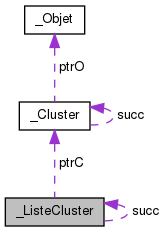
\includegraphics[scale=0.5]{images/struct_liste_cluster.png}
\caption{Graphe de collaboration de la structure ListeCluster (\textit{Cluster First Root Second})}
\end{figure} 


\subsection{Cluster}

Ci-dessous la représentation de la structure Cluster. 
\begin{figure}[H]

\begin{tabbing}
\texttt{Cluster = \^\,Place;} \\
\texttt{Place =} \= \texttt{enregistrement} \\
\> \texttt{ptrO : Objet;} \\
\> \texttt{succ : Cluster;} \\
\> \texttt{fin;}\\
\end{tabbing}

\caption{Représentation de la structure Cluster}
\end{figure}

\paragraph{}
La structure Cluster est une liste cha\^inée à l'aide de l'attribut "succ". Chaque cellule pointe vers une autre cellule de la structure et vers un élément de type Objet.
Ci-dessous, le graphe de collaboration de la structure Cluster.  

\begin{figure}[H]
\center
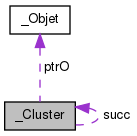
\includegraphics[scale=0.5]{images/struct_cluster.png}
\caption{Graphe de collaboration de la structure Cluster}
\end{figure} 

\subsection{Objet}
\label{subsec:Objet.h}
La structure Objet peut-\^etre représentée de la manière suivante : 
\begin{figure}[H]
\begin{tabbing}
\texttt{Objet = \^\,Element;}\\
\texttt{Element =} \= \texttt{enregistrement}\\
\> \texttt{idObjet : Entier non signé;} \\
\> \texttt{coordx : Entier;} \\
\> \texttt{coordy : Entire;} \\
\> \texttt{poids : Entier non signé;} \\
\> \texttt{trie : Bool;} \\
\> \texttt{fin;}\\
\end{tabbing}

\caption{Représentation de la structure Objet}
\end{figure}

\paragraph{}
Un élément de la structure Objet représente un produit. Pour chaque produit, on indiquera : 
\begin{itemize}
\item[•]\textbf{l'identifiant} : idObjet
\item[•]\textbf{son coordonnée x} : coordx
\item[•]\textbf{son coordonnée y} : coordy 
\item[•]\textbf{son poids} : poids
\item[•]\textbf{s'il a déjà été trié} : trie
\end{itemize}


\section{Architecture du programme}

\paragraph{}
Le programme est axé autour d'un fichier principal appelé par le \textit{main}, \textit{ClusterFirst.h}. Dans le \textit{main} sont aussi inclus les différentes structures citées auparavant(\ref{subsec:struct} page \pageref{subsec:struct}) ainsi que différents fichier de la librairie C. 
On peut représenter le graphe des dépendances par inclusion du \textit{main} de la façon suivante : 

\begin{figure}[H]
	\center
	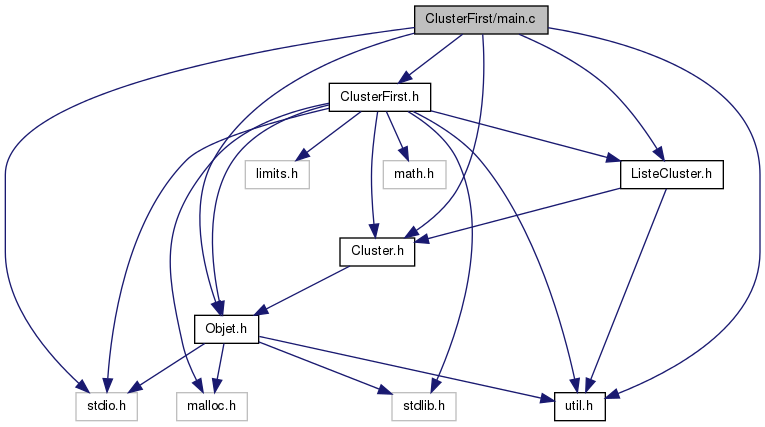
\includegraphics[scale=0.5]{images/main_inclusion.png}
	\caption{Graphe des dépendances par inclusion de \textit{main.c}}
\end{figure} 

\paragraph{}
Le main appel trois fonctions : 
\begin{itemize}
\item[•]\textbf{init} : Permet de récupérer les paramètres(capacité maximum du chariot ainsi que le fichier texte contenant les informations sur les produits, c'est à dire le carnet de commande) et affiche un message d'erreur si aucuns paramètres n'a été passé.
\item[•]\textbf{remplissageCluster}\footnote{cf algorithme n\degre \ref{algo:remplissageCluster}} : Découpe le carnet de commande en cluster.
\item[•]\textbf{trieListeCluster} \footnote{cf algorithme n\degre \ref{algo:trieListeCluster}}: Trie chaque cluster crée avec remplissageCluster pour que le chariot effectue l'itinéraire le plus court possible.
\end{itemize}

\paragraph{}
Le graphe d'appel du \textit{main} (ci-dessous), montre tous les appels de fonction effectuer à partir celui-ci à travers les trois fonctions citées précédemment.

\begin{figure}[H]
	\center
	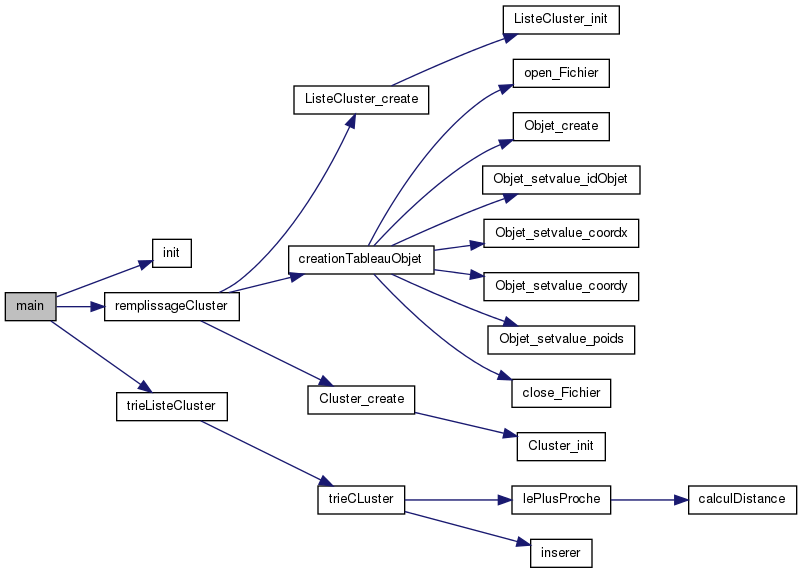
\includegraphics[scale=0.5]{images/main_appel.png}
	\caption{Graphe d'appel de la fonction \textit{main}}
\end{figure}

\section{Algorithmes}

\paragraph{}
Dans cette section, les principaux différents algorithmes seront décrits.

\subsection{Remplissage des clusters}

\paragraph{}
Afin de créer une liste de clusters, il faut tout d'abord remplir la structure Objet avec les informations des produits. Pour cela on va utiliser la fonction \textit{creationTableauObjet} dont voici l'algorithme : 

\begin{algorithm}[H]
\caption{Creation d'un tableau de pointeur vers des Objets : \textit{creationTabObjet}}
\label{algo:creationTabObjet}
\algsetup{indent=3em}
\begin{algorithmic}[1]
\REQUIRE { %
 entrées : $filename$ : fichier texte, $nb\_lignes$ : nombre de lignes, $cap\_max$ : capacité maximum du chariot}
\ENSURE { sortie : $tabObjet$ : le tableau de pointeur vers des Objets, $nb\_lignes$ : le nombre de produits}

\STATE $file \leftarrow ouvrirFichier(filename)$ 
\COMMENT{ouverture du fichier}
\STATE $allouer(tabObjet)$
\COMMENT{ allocation mémoire de $tabObjet$ }
\STATE $lire(file, nb\_lignes)$
\COMMENT{lecture de la première ligne et récupération du nombre d'item dans $nb\_lignes$}
\FOR[parcours du fichier ]{$indice$ \textbf{de} 1 \textbf{à} $nb\_lignes$ \textbf{faire}}
	\STATE $lire(file, idObjet, coordx, coordy, poids)$
	\COMMENT{lecture d'une ligne}
	\STATE $creer(Objet)$
	\COMMENT{allocation mémoire et initialisation de $Objet$}
	\STATE $Objet\uparrow idObjet \leftarrow idObjet$
	\STATE $Objet\uparrow coordx \leftarrow coordx$
	\STATE $Objet\uparrow coordy \leftarrow coordy$
	\STATE $Objet\uparrow poids \leftarrow poids$
	\IF[vérifie que le poids des produits est inférieur à la capacité du chariot]{($Objet\uparrow poids < cap\_max$)}
	\STATE $afficher($Erreur poids produits trop élévé$)$
	\STATE $exit$
	\ENDIF
	\STATE $tabObjet[indice] \leftarrow Objet$
\ENDFOR
\STATE $fermetureFichier(file)$
\COMMENT{fermeture du flux}
\RETURN $tabObjet$

\end{algorithmic}
\end{algorithm}

\paragraph{}
Après l'allocation de la structure Objet, on peut remplir les différents clusters à partir de la fonction \textit{remplissageCLuster}. L'algorithme de cette fonction est le suivant : 

\begin{algorithm}[H]
\caption{Remplissage des clusters : \textit{remplissageCluster}}
\label{algo:remplissageCluster}
\algsetup{indent=3em}
\begin{algorithmic}[1]
\REQUIRE { %
 entrées : $filename$ : fichier texte,$cap\_max$ : capacité maximum du chariot}
\ENSURE { sortie : $listeCluster$ : pointeur sur la tête de la liste de clusters}

\STATE $creer(listeCLuster)$ 
\COMMENT{allocation mémoire et création de $listeCluster$}
\STATE $tabObjet\leftarrow creationTabObjet(filename, nb\_lignes, cap\_max)$
\COMMENT{appel de la fonction $creationTabObjet$ }
\STATE $listeCLusterHead\leftarrow listeCluster$
\COMMENT{fait pointer la tête de liste vers $listeCluster$}
\FOR[Parcours de tabObjet ]{$indice$ \textbf{de} 1 \textbf{à} $nb\_lignes$ \textbf{faire}}
		\STATE $Objet \leftarrow tabObjet[indice]$	
		\COMMENT{$Objet$ reçoit le pointeur vers un Objet de la case $indice$ de $tabObjet$}
		\STATE $newCap \leftarrow listeCluster\uparrow cap + Objet\uparrow poids$
		\COMMENT{addition de la capacité du cluster en cours et du poids de l'objet a ajouter}
		\WHILE{(($cap\_max < newCap)\AND (listeCluster\uparrow succ \neq NULL$))}
			\STATE $listeCluster \leftarrow listeCluster\uparrow succ$
			\STATE $newCap \leftarrow listeCluster\uparrow cap + Objet\uparrow poids$
		\ENDWHILE
		\IF[s'il y a de la place pour ajouter l'objet]{$newCap \leq cap\_max$}
			\STATE $clusterTmp \leftarrow listeCluster\uparrow ptrC$
			\COMMENT{$clusterTmp$ pointe vers la tête de liste du cluster}
			\WHILE{($clusterTmp\uparrow succ \neq NULL$)} 
				\STATE $clusterTmp \leftarrow clusterTmp\uparrow succ$
				\COMMENT{parcours du cluster jusqu'à la fin}
			\ENDWHILE
			\STATE $creer(cluster)$
			\COMMENT{allocation mémoire et initialisation de $cluster$}
			\STATE $clusterTmp\uparrow succ \leftarrow cluster$
			\STATE $cluster\uparrow ptrO \leftarrow Objet$
			\STATE $listeCluster\uparrow cap \leftarrow newCap$
		\ELSE[si pas assez de place dans aucun cluster déjà existant]
			\STATE $creer(listeCLusterTmp)$
			\COMMENT{allocation mémoire et initialisation de $listeClusterTmp$}
			\STATE $listeCluster\uparrow succ \leftarrow listeClusterTmp$
			\STATE $listeCluster \leftarrow listeClusterTmp$
			\STATE $listeCluster\uparrow cap \leftarrow objet\uparrow poids$
			\STATE $creer(cluster)$
			\COMMENT{allocation mémoire et initialisation de $cluster$}
			\STATE $listecLuster\uparrow ptrC \leftarrow cluster$
			\STATE $cluster\uparrow ptrO \leftarrow objet$
		\ENDIF
		\IF{($listecluster\uparrow cap = cap\_max$)}
			\STATE $listeCLuster\uparrow fini \leftarrow TRUE$
		\ENDIF
\ENDFOR
\RETURN $listeClusterHead$


\end{algorithmic}
\end{algorithm}

\subsection{Trie des clusters}

\paragraph{}
Lorsque la liste des clusters est crée, il faut ensuite trier chacun d'eux pour que l'itinéraire du chariot soit le plus court possible. Pour ce faire, nous avons réaliser trois algorithmes :
\begin{enumerate}
\item\textit{trieListeCluster} \footnote{cf algorithme n\degre \ref{algo:trieListeCluster}} : Permet de trier la liste des Clusters
\item\textit{trieCluster}\footnote{cf algorithme n\degre \ref{algo:trieCluster}} : Trie chaque cluster
\item\textit{lePlusProche} \footnote{cf algorithme n\degre \ref{algo:lePlusProche}} : Cherche l'objet le plus proche de celui passer en paramètre dans son cluster
\end{enumerate}

\begin{algorithm}[H]
\caption{Trie de la liste des clusters : \textit{trieListeCluster}}
\label{algo:trieListeCluster}
\algsetup{indent=3em}
\begin{algorithmic}[1]
\REQUIRE { %
 entrées : $listeCluster$ : liste des clusters}
%\ENSURE { sortie : $listeCluster$ : pointeur sur la tête de la liste de clusters}

\WHILE{($listeCluster \neq NULL$)}
	\STATE $dist \leftarrow trieCluster(listeCluster\uparrow ptrC)$
	\COMMENT{retourne la distance à effectuer par le chariot dans le cluster}
	\STATE $listeCluster \leftarrow listeCluster\uparrow succ$
	\STATE $distTotal \leftarrow distTotal + dist$
\ENDWHILE
\STATE $afficher(la distance a parcourir par le chariot est : distTotal)$

\end{algorithmic}
\end{algorithm}

\begin{algorithm}[H]
\caption{Trie d'un cluster : \textit{trieCluster}}
\label{algo:trieCluster}
\algsetup{indent=3em}
\begin{algorithmic}[1]
\REQUIRE { %
 entrées : $head$ : pointeur vers la tête de la liste du cluster}
\ENSURE { sortie : $distTotal$ : distance à parcourir par le chariot dans le cluster}

\STATE $enCours \leftarrow head$
\WHILE{($enCours\uparrow succ \neq NULL$)}
	\STATE $comp++$
	\COMMENT{compte le nombre d'item du cluster}
\ENDWHILE
\STATE $enCours \leftarrow head$
\WHILE{($enCours \neq NULL$)}
	\STATE $clusterTmp \leftarrow lePlusProche(head, enCours, dist, compt)$
	\COMMENT{retourne le cluster le plus proche de enCours}
	\STATE $listeCluster \leftarrow listeCluster\uparrow succ$
	\STATE $distTotal \leftarrow distTotal + dist$
	\STATE $inserer(enCours, clusterTmp, head)$
	\COMMENT{insère la cellule clusterTmp avant celle d'enCours et refait le chainage de la liste}
	\STATE $enCours \leftarrow clusterTmp$
\ENDWHILE
\STATE $afficher(la distance a parcourir par le chariot est : distTotal)$
\RETURN $distTotal$

\end{algorithmic}
\end{algorithm}


\begin{algorithm}[H]
\caption{Cherche le cluster le plus proche : \textit{lePlusProche}}
\label{algo:lePlusProche}
\algsetup{indent=3em}
\begin{algorithmic}[1]
\REQUIRE { %
 entrées : $head$ : pointeur vers la tête de la liste du cluster, $enCours$ : pointeur vers le cluster courant, $distmin$ : distance minimum, $compt$ : nombre de cellule du cluster}
\ENSURE { sortie : $plusProche$ : cluster le plus proche de enCours, $distmin$ : distance entre $plusProche$ et $enCours$}

\STATE $ObjetCourant \leftarrow enCours\uparrow ptrO$
\STATE $minDist \leftarrow infini$
\STATE $cluster \leftarrow head$
\FOR[parcours du cluster]{$indice$ \textbf{de} 1 \textbf{à} $compt$ \textbf{faire}}
	\STATE $objetTmp \leftarrow cluster\uparrow ptrO$
	\IF[si $objetTmp$ n'a pas déjà été trié et s'il est différent de $objet$]{(($objetTmp\uparrow trie = FALSE) \AND (objetTmp \neq objet$))}
		\STATE $dist \leftarrow calculDistance(objet\uparrow coordx, objet\uparrow coordy, objetTmp\uparrow coordx, objetTmp\uparrow coordy)$
		\COMMENT{calcul la distance euclidienne entre $objetTmp$ et $objet$}
		\IF{($dist < minDist$)}
			\STATE $minDist \leftarrow dist$
			\STATE $plusProche \leftarrow cluster$
		\ENDIF
	\ENDIF
	\STATE $cluster \leftarrow cluster\uparrow succ$
\ENDFOR
\RETURN $plusProche$
\end{algorithmic}
\end{algorithm}

%%%%%%%%%%%%%%%%%%%% CHAPITRE 3 %%%%%%%%%%%%%%%%%%%%%%

\chapter{Root First Cluster Second}

\paragraph{}
Ce chapitre a pour objectif de présenter l'heuristique \textit{Root First Cluster Second}.

\section{Structure de données}

Pour cette heuristique, nous avons repris les même structure de données que pour \textit{Cluster First Root Second} avec quelques modifications.

\paragraph{}
Les différentes structures utilisées pour cette heuristique sont dans les fichiers suivants :
\begin{itemize}
	\item[•]\textit{util.h}
	\item[•]\textit{ListeCluster.h}
	\item[•]\textit{ListeObjet.h}
	\item[•]\textit{Objet.h}
\end{itemize}

\paragraph{}
Les structures définies dans \textit{util.h}\footnote{voir \ref{subsec:util.h} page \pageref{subsec:util.h}} et \textit{Objet.h} \footnote{voir \ref{subsec:Objet.h} page \pageref{subsec:Objet.h}} sont les mêmes que celle de \textit{Cluster First Root Second}. 

\subsubsection{ListeCluster}

\paragraph{}
ListeCLuster est une liste chainée qui peut être représentée de la manière suivante : 

\begin{figure}[H]

\begin{tabbing}
\texttt{ListeCluster = \^\,Place;} \\
\texttt{Place =} \= \texttt{enregistrement} \\
\> \texttt{ptrLO : ListeObjet;} \\
\> \texttt{succ : ListeClutser;} \\
\> \texttt{fin; } \\
\end{tabbing}

\caption{Représentation de la structure ListeCluster (\textit{Root First Cluster Second})}
\end{figure}

\paragraph{}
Cette structure est une liste chainée de pointeurs vers la tête de la liste d'objets. Elle permet de pouvoir gérer facilement chaque liste d'objets correspondant à un cluster. 
Ci-dessous une représentation du graphe de collaboration de la structure ListeCluster.


\begin{figure}[H]
	\center
	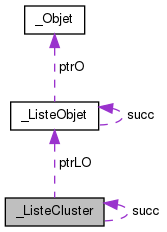
\includegraphics[scale=0.5]{images/struct_listeClusterRF.png}
	\caption{Graphe de collaboration de la structure ListeCLuster (\textit{Root First Cluster First})}
\end{figure} 

\subsubsection{ListeObjet}

\paragraph{}
La structure ListeObjet a été défini pour gérer chaque cluster. C'est une liste chainée de pointeurs vers des Objets (voir \ref{subsec:Objet.h}). Cette structure a pour représentation la figure ci-dessous : 

\begin{figure}[H]

\begin{tabbing}
\texttt{ListeObjet = \^\,Place;} \\
\texttt{Place =} \= \texttt{enregistrement} \\
\> \texttt{ptrO : Objet;} \\
\> \texttt{succ : ListeObjet;} \\
\> \texttt{fin; } \\
\end{tabbing}

\caption{Représentation de la structure ListeObjet}
\end{figure}

\paragraph{}
Chaque cellule de la structure a pour attribut un pointeur vers un Objet et un pointeur vers la cellule suivante, comme le montre le graphe de collaboration suivant : 

\begin{figure}[H]
\center
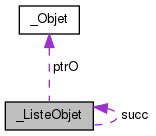
\includegraphics[scale=0.5]{images/struct_listeobjet.png}
\caption{Graphe de collaboration de la structure ListeObjet}
\end{figure} 

\section{Architecture du programme}

\paragraph{}
Le code source du programme se situe dans le fichier \textit{RootFirst.c}. Celui est inclus dans le fichier \textit{main.c}. 
Pour plus de clarté sur les inclusions \textit{main}, voici le graphe des dépendances par inclusion de celui-ci : 


\begin{figure}[H]
\center
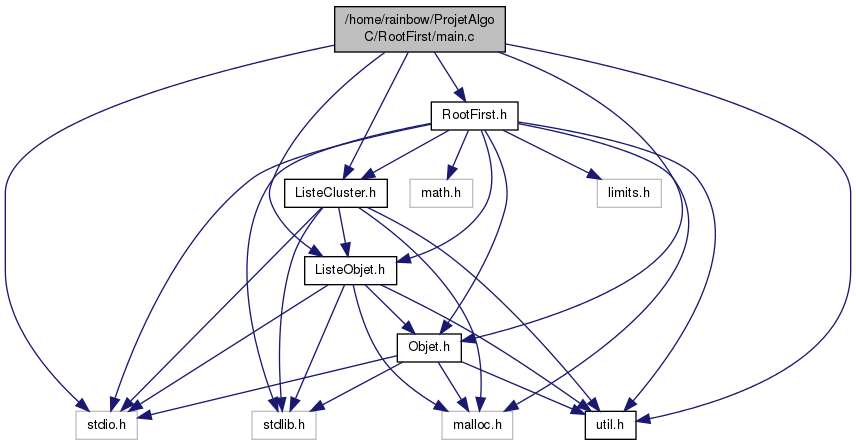
\includegraphics[scale=0.5]{images/main_inclusionRF.png}
\caption{Graphe des dépendances par inclusion de \textit{main.c} (\textit{Root First Cluster Second})}
\end{figure} 

\paragraph{}
Le main fait appel à trois fonctions : 
\begin{itemize}
	\item[•]\textbf{init} : Cette fonction a pour objectif de récupérer les paramètres lors de l'exécution du programme. Il y a deux paramètres à fournir le capacité maximum du chariot et le fichier texte avec les informations sur les produits. Si ce n'est pas le cas, la fonction renvoie une erreur.
	\item[•]\textbf{trieTabObjet} : Après la création d'un tableau de pointeurs vers des Objets contenant les informations relatives aux produits de la commande, cette fonction trie ce tableau de façon à obtenir l'itinéraire le plus court pour le chariot. Elle renvoie une liste d'Objets. 
	\item[•]\textbf{creationListeCLuster} : Cette fonction découpe la liste d'objets obtenue avec la fonction précédente en cluster ne dépassant pas la capacité maximum du chariot.
\end{itemize}
\paragraph{}
Ces appels de fonction dans le \textit{main} peuvent être schématisé avec un graphe d'appel du \textit{main}.


\begin{figure}[H]
\center
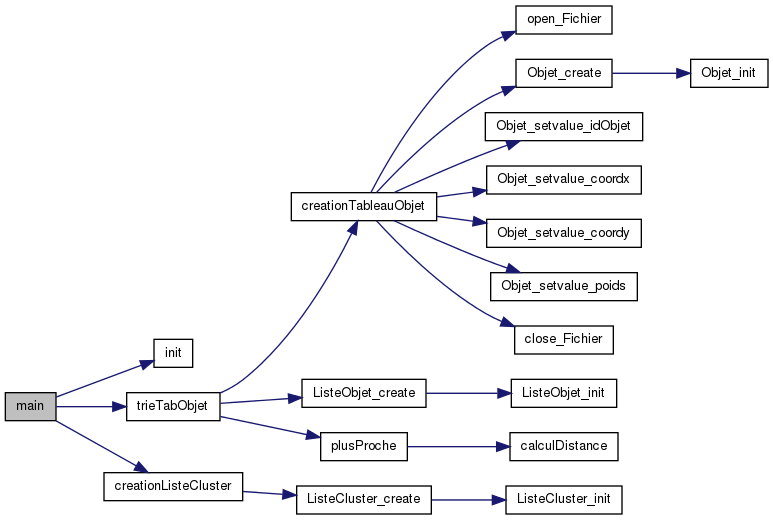
\includegraphics[scale=0.5]{images/main_appelRF.png}
\caption{Graphe d'appel de la fonction main (\textit{Root First Cluster Second})}
\end{figure} 


\section{Algorithmes}

\paragraph{}
Cette section a pour objectif de présenter les principaux algorithmes du programme \textit{Root First Cluster Second}. Les algorithmes des fonctions \textit{creationtabObjet} et \textit{lePlusProche} ne seront pas explicité car ils sont similaires à ceux du programme \textit{Cluster First Root Second}.

\subsection{Trie des items}

\paragraph{}
La méthode \textit{Root First Cluster Second} consiste à tout d'abord trouver l'itinéraire que devra effectuer le chariot puis ensuite à découper celui-ci à chaque fois que le chariot aura atteint sa capacité maximale. 

\paragraph{}
Ce premier algorithme permet de trier les objets pour obtenir le meilleur itinéraire. Il renvoi un pointeur vers la tête de la liste de structure ListeObjet. 

\begin{algorithm}[H]
\caption{Creation d'une liste de pointeurs vers des Objets triée : \textit{trieTabObjet}}
\label{algo:creationTabObjet}
\algsetup{indent=3em}
\begin{algorithmic}[1]
\REQUIRE { %
 entrées : $filename$ : fichier texte, $cap\_max$ : capacité maximum du chariot}
\ENSURE { sortie : $ListeObjet$ : listeObjets trié}

\STATE $tabObjet \leftarrow crationTabObjet(filename, nb\_lignes, cap\_max)$
\COMMENT{crée un tableau de pointeur vers des Objets et récupère avec $nb\_lignes$ le nombre d'item}
\STATE $objetEnCours \leftarrow tabObjet[1]$
\STATE $creer(listeObjetHead)$
\COMMENT{allocation et initialisation de $listeObjetHead$}
\STATE $lsiteObjet \leftarrow listeObjetHead$
\FOR[Création de la liste]{$indice$ \textbf{de} 1 \textbf{à} $nb\_lignes-1$ \textbf{faire}}
	\STATE $creer(listeObjetTmp)$
	\COMMENT{allocation et initialisation de $listeObjetTmp$}
	\STATE $listeObjet\uparrow succ \leftarrow listeObjetTmp$
	\STATE $listeObjet \leftarrow listeObjet\uparrow succ$
\ENDFOR
\STATE $listeObjet \leftarrow listeObjetHead$
\COMMENT{met le pointeur de la liste sur la tête}
\WHILE{($listeObjet \neq NULL$)}
	\STATE $objetPlusProche \leftarrow lePlusProche(objetEnCours, tabObjet,nb\_lignes, dist)$ 
	\COMMENT{cherche l'objet le plus proche d'$objetEnCours$ et retourne la distance les séparant}
	\STATE $listeObjet\uparrow ptrO \leftarrow objetPlusProche$
	\STATE $objetEnCours \leftarrow objetPlusProche$
	\STATE $distTotal \leftarrow distTotal + dist$
	\STATE $listeObjet \leftarrow listeObjet\uparrow succ$
\ENDWHILE
\RETURN $listeObjetHead$

\end{algorithmic}
\end{algorithm}

\subsection{Découpage en clusters}

\paragraph{}
La fonction \textit{creationListeCluster} découpe la liste d'Objets (listeObjet), crée avec la fonction \textit{trieTabObjet}, en cluster de capacité inférieur ou égal à la capacité maximum du chariot. 

\begin{algorithm}[H]
\caption{Creation d'une liste de pointeurs vers des liste d'Objets : \textit{creationListeCluster}}
\label{algo:creationTabObjet}
\algsetup{indent=3em}
\begin{algorithmic}[1]
\REQUIRE { %
 entrées : $listeObjet$ : pointeur vers la tête de la liste d'Objets, $cap\_max$ : capacité maximum du chariot}

\STATE $cap \leftarrow 0$
\STATE $listeObjetHead \leftarrow listeObjet$
\STATE $creer(listeCluster$
\COMMENT{allocation et initialisation de $listeCluster$}
\WHILE{($listeObjet \neq NULL$)}
	 \STATE $objet \leftarrow listeObjet\uparrow ptrO$
	 \STATE $cap \leftarrow cap + obket\uparrow poids$
	 \IF[si $listeObjet$ n'est pas le dernier élément de la liste]{($listeObjet\uparrow succ \neq NULL$)}
	 	\STATE $listeObjetTmp \leftarrow listeObjet\uparrow succ$
	 	\STATE $objetTmp \leftarrow listeObjetTmp\uparrow ptrO$
	 	\IF[si $ObjetTmp$ ne peut pas rentrer dans le cluster]{(($cap +objetTmp\uparrow poids) > cap\_max$)}
	 		\STATE $creer(listeClusterTmp)$
	 		\STATE $listeCLuster\uparrow ptrLO \leftarrow listeObjetHead$
	 		\COMMENT{le cluster pointe vers la tête de la liste d'Objets}
	 		\STATE $listeObjet\uparrow NULL$
	 		\COMMENT{défini la fin de liste d'Objets dans le cluster}
	 		\STATE $listeObjetHead \leftarrow listeObjetTmp$
	 		\COMMENT{la liste d'Objets du prochain cluster pointera vers $listeObjetTmp$}
	 		\STATE $listeObjet \leftarrow listeObjetTmp$
	 		\STATE $listeCluster\uparrow succ \leftarrow listeCLusterTmp$
	 		\STATE $listeCluster \leftarrow listeCluster\uparrow succ$
	 		\STATE $cap \leftarrow 0$
	 		\COMMENT{remet la capacité du prochain cluster à 0}
	 	\ELSE
	 		\STATE $listeObjet \leftarrow listeObjet\uparrow succ$
	 	\ENDIF
	 \ELSE[cas pour le dernier élément de listeObjet]
	 	\STATE $listeCluster\uparrow ptrLO \leftarrow listeOBjetHead$
	 	\STATE $listeObjet \leftarrow listeObjet\uparrow succ$
	 \ENDIF
\ENDWHILE
	 

\end{algorithmic}
\end{algorithm}




%%%%%%%%%%%%%%%%%%%%%%% CHAPITRE 4 %%%%%%%%%%%%%%%%%%

\chapter{Test des différentes heuristiques}
\label{chap:test}

\section{Mise en place des tests}

\paragraph{}
Pour mettre en place les tests sur les heuristiques, il faut tout d'abord déterminer les données du problèmes qui sont ici, la capacité maximum du chariot ($cap$) et le nombre de produits de la commande.

\paragraph{}
Soit $n$ le nombre d'item, le couple de coordonnées($x,y$) et $p$ le poids, on peut définir la propriété suivante : 
\begin{align}
\forall i\in [1,n], \exists
\left\{
  \begin{array}{rcr}
   (x_{i},y_{i}) \\
     p_{i} \\
  \end{array}
\right.
\end{align}

\paragraph{}
Lors de la réalisation des tests, des fichiers de produits ou instances seront généré. On prendra $p_{i}\in [1,10]$ et $(x_{i},y_{i}) \in [-100, 100]$.

\paragraph{}
Seront pris en compte les ensembles de valeurs suivant pour déterminer les jeux de tests à réaliser : 
\begin{itemize}
	\item[•]$n \in \{100, 200\}$
	\item[•]$cap \in \{20, 30\}$
\end{itemize} 

\paragraph{}
Il y a quatre jeux de tests à effectuer avec en paramètre le couple ($n, cap$) : (100, 20), (100,30), (200, 20) et (200, 30).
Chaque jeu de tests sera testé sur vingt instances générées aléatoirement. Une instance sera lancée deux fois, une fois par heuristique. 

\section{Résultats des tests}

\subsection{Dominance}

\paragraph{}
Après réalisation des quatre jeux de test, on remarque que  
\textit{Root First Cluster Second} domine toujours \textit{Cluster Root First Second}. 

\begin{table}[H]
\centering
\begin{tabular}{|c|c|c|}
\hline 
($n,cap$) & \textit{Cluster First Root Second} & \textit{Root First Cluster Second} \\ 
\hline 
(100, 20) & 0/20 & 20/20 \\ 
\hline 
(100, 30) & 0/20 & 20/20 \\
\hline 
(200, 20) & 0/20 & 20/20 \\ 
\hline 
(200, 30) & 0/20 & 20/20 \\ 
\hline 
\end{tabular}
\caption{Tableau de dominances} 
\end{table}

\paragraph{}
Ce tableau signifie que pour le jeu de test (100, 20) par exemple, l'heuristique \textit{Root First Cluster Second} sur vingt instances a renvoyé vingt fois une distance inférieur à celle de \textit{Cluster First Root Second}. 

\subsection{Gap}

\paragraph{}
Nous avons calculé le gap minimum, maximum et moyen pour chaque jeu de tests de chaque heuristique. 
Pour cela, nous avons utilisé les formules suivantes lorsque \textit{Cluster First Root Second} domine :  


\begin{align}
gap_{min} = \min_{1 \leqslant i \leqslant 20}(\frac{distRoot - distClsuter}{distCluster} * 100) \\
gap_{max} = \max_{1 \leqslant i \leqslant 20}(\frac{distRoot - distClsuter}{distCluster} * 100) \\
gap_{moy} = \frac{\displaystyle\sum_{i=1}^{nbr\, de\, dominances}(\frac{distRoot - distClsuter}{distCluster} * 100)}{nbr\, de\, dominances}
\end{align}

\paragraph{}
Et lorsque \textit{Root First Cluster Second} domine : 

\begin{align}
gap_{min} = \min_{1 \leqslant i \leqslant 20}(\frac{distCluster - distRoot}{distRoot} * 100) \\
gap_{max} = \max_{1 \leqslant i \leqslant 20}(\frac{distCluster - distRoot}{distRoot} * 100) \\
gap_{moy} = \frac{\displaystyle\sum_{i=1}^{nbr\, de\, dominances}(\frac{distCluster - distRoot}{distRoot} * 100)}{nbr\, de\, dominances}
\end{align}

\paragraph{}
Ces calculs permettent d'obtenir le tableau de résultats suivant : 

\begin{table}[H]
\centering
\begin{tabular}{|c|c|c|c|c|c|c|}
\hline
 & \multicolumn{3}{c|}{dominance de \textit{Cluster First root Second}} & \multicolumn{3}{c|}{dominance de \textit{Root First Cluster Second}} \\ 
\hline 
($n, cap$) & $gap_{min}$ & $gap_{max}$ & $gap_{moy}$ & $gap_{min}$ & $gap_{max}$ & $gap_{moy}$ \\ 
\hline 
(100, 20) & -65 & -46 & 0 & 87 & 191 & -1146 \\ 
\hline 
(100, 30) & -54 & 8 & 8 & -8 & 119 & -37 \\ 
\hline 
(200, 20) & -74 & -63 & 0 & 175 & 295 & -1401 \\ 
\hline 
(200, 30) & -65 & -37 & 0 & 59 & 193 & -1113 \\ 
\hline 
\end{tabular} 
\caption{Tableau de résultats des $gap_{min}$, $gap_{max}$ et $gap_{moy}$} 
\end{table}

\paragraph{}
Malgré le fait que les résultats des tests ne soient pas concluants, l'on peut quand même remarquer sur le tableau que \textit{Root First Cluster Second} semble avoir un  pourcentage de dominance plus élevé.

\paragraph{}
Les résultats obtenus dans le tableau précédent peuvent être généralisé avec la formule suivante : 


Soit $H_{k}$ l'heuristique $k$ et $dist$ la distance retournée lors de l'exécution d'un heuristique alors pour chaque résultat des instances d'un jeu de test on a $$ gap_{H_{k}} =  \frac{\displaystyle\sum_{j=1}^{20}(\frac{dist_{j\, H_{k}} - dist_{j}^{best}}{dist_{j}^{best}} * 100)}{20}$$


\begin{table}[H]
\centering
\begin{tabular}{|c|c|c|}
\hline 
($n,cap$) & \textit{Cluster First Root Second} & \textit{Root First Cluster Second} \\ 
\hline 
(100, 20) & 3 & 0 \\ 
\hline 
(100, 30) & 2 & -219 \\
\hline 
(200, 20) & 3 & 0 \\ 
\hline 
(200, 30) & 2 & 0 \\ 
\hline 
\end{tabular}
\caption{Tableau de résultats général des gaps} 
\end{table}

\subsection{Temps d'exécution}

\paragraph{}
Les temps de calcul avec 100 et 200 items étant très infimes, nous avons refait les tests des deux heuristiques avec $n \in \{10000, 20000\}$. 

\paragraph{}
La moyenne des temps d'exécutions de chaque heuristique pour chaque jeu de tests ont été calculé avec la formule suivante : 

\begin{align}
 tempsMoy = \frac{\displaystyle\sum_{i=0}^{20}temps_{i}}{20}
\end{align}

\paragraph{}
Voici le tableau des résultats obtenus : 

\begin{table}[H]
\centering
\begin{tabular}{|c|c|c|}
\hline 
($n,cap$) & \textit{Cluster First Root Second} & \textit{Root First Cluster Second} \\ 
\hline 
(10000, 20) & 0.05 & 1.70 \\ 
\hline 
(10000, 30) & 0.05 & 1.72 \\
\hline 
(20000, 20) & 0.11 & 7.20 \\ 
\hline 
(20000, 30) & 0.11 & 7.80 \\ 
\hline 
\end{tabular}
\caption{Tableau des temps d'exécutions (en secondes)} 
\end{table}

\paragraph{}
Le temps d'exécution de \textit{Root First Cluster Second} est plus long que celui de \textit{Cluster First Root Second} mais sans qu'il y ait une grande différence d'écart entre les deux à faible niveau. Mais sur de plus grand jeu l'écart est plus visible.

\paragraph{}
Le changement du nombre d'items est visible avec les résultats pour les deux heuristiques. Le temps d'exécution augmente peu lors de ce changement pour \textit{Cluster First Root Second} contrairement à \textit{Root First Cluster Second}. La modification de la capacité du chariot n'a visiblement aucune influence sur \textit{Cluster First Root Second} à l'inverse de \textit{Root First Cluster Second} dont le temps d'exécution augmente légèrement.

%%%%%%%%%%%%%%%%%%%% CONCLUSION %%%%%%%%%%%%%%%%%%%%%%

\chapter{Conclusion}


\paragraph{}
\`A ce stade du projet, l'heuristique \textit{Root First Cluster Second} semble être la meilleur mais il manque des paramètres à prendre en compte. Pour le moment, l'heuristique \textit{Cluster First Root Second} renvoie toujours des résultats beaucoup plus grand que \textit{Root First Cluster Second} mais sur de grandes instances s'exécute nettement plus vite.

\paragraph{}
Ce projet pourrait être améliorer en optimisant chaque heuristique et en tenant compte d'une structure précise d'un entrepôt ou en ajoutant plusieurs chariots. 

\paragraph{}
Tout au long de ce projet, nous avons dû explorer différentes pistes d'algorithmes pour chaque heuristique. Chercher comment avec la méthode \textit{Cluster First Root Second}, créer les différents clusters du carnet de commande pour notre chariot ou bien choisir les bonnes structures pour les deux heuristiques, nous ont permis de nous améliorer. 

%\annexes

\end{document}

